\chapter{Detectability in Spectroscopic Surveys}
\label{chapter:snreuclid}
%
The Fourier galaxy bispectrum is complex, with the imaginary part arising from leading-order relativistic corrections, due to Doppler, gravitational redshift  and related line-of-sight effects  in redshift space. The detection of the imaginary  part of the bispectrum is potentially a smoking gun signal of relativistic contributions.  We investigate whether next-generation spectroscopic surveys could make such a detection. For a Stage IV spectroscopic $H\alpha$ survey similar to Euclid, we find that  the cumulative signal to noise of this relativistic signature  is $\mathcal{O}(10)$. 
{Long-mode relativistic effects couple to  short-mode Newtonian effects in the galaxy bispectrum, but not in the galaxy power spectrum.
This is  the basis for detectability of relativistic effects in the bispectrum of a single galaxy survey, whereas the power spectrum requires multiple galaxy surveys to detect the corresponding signal.}
%
%
%-----------------------------------
%
%
\section{Introduction}
%
%
%
%------------------------------------------------
%
%
\section{Signal-to-Noise}
%
The signal-to-noise ratio (SNR) for the bispectrum  at redshift $z$ is given in the Gaussian approximation of uncorrelated triangles by \cite{Scoccimarro:2003wn}
\begin{equation}
\bigg[\frac{S}{N}(z)\bigg]^{2} = 
\sum_{k_a,\,\mu_{1},\,\varphi}\,\frac{1}{{\mathrm{Var}} [{B_{g}}(z, k_a,\mu_{1},\varphi)]}
\,B_{g}(z, k_{a},  \mu_{1},\varphi)\,B^*_{g}(z, k_a, \mu_{1},\varphi)
\end{equation} 
where we have introduced the complex conjugate $B^*_{g}$ since the bispectrum  has an imaginary correction. {Here ${\mathrm{Var}} [{B_{g}}]$ is the variance  of the bispectrum estimator
 \cite{Chan:2016ehg}:
\begin{equation} 
\hat{B}_g(z,\bm{k}_a) = \frac{k_{\mathrm{f}}^3}{V_{123}}\int_{\bm{k}_a}\ud^3\bm{q}_1\, \ud^3\bm{q}_2 \,\ud^3\bm{q}_3\,\delta^{{\mathrm{Dirac}}}(\bm{q}_1+\bm{q}_2+\bm{q}_3)\, \delta_g(z,\bm{q}_1) \delta_g(z,\bm{q}_2) \delta_g(z,\bm{q}_3) \,,
\end{equation}
where integration is over the shells $k_a-\Delta k/2\leq q_a \leq k_a+\Delta k/2$ and  the shell volume is
$V_{123}=\int_{\bm{k}_a}\ud^3\bm{q}_1\, \ud^3\bm{q}_2 \,\ud^3\bm{q}_3\,\delta^{{\mathrm{Dirac}}}(\bm{q}_1+\bm{q}_2+\bm{q}_3)$.}


In the Newtonian approximation, the Gaussian variance can be given as \cite{Scoccimarro:2003wn, Karagiannis:2018jdt}
\begin{equation}
{{\mathrm{Var}} [{B_{g}}(z, k_a,\mu_{1},\varphi)]}
=s_B\, \frac{\pi k_{\mathrm{f}}(z)^3}{k_1k_2k_3 (\Delta k)^3}\,\frac{N_{\mu_1}N_\varphi}{\Delta \mu_1 \Delta \varphi} \, \tilde{P}_{g{\mathrm{N}}}(z,k_{1},\mu_{1}) \tilde{P}_{g{\mathrm{N}}}(z,k_{2},\mu_{2})\tilde{P}_{g{\mathrm{N}}}(z,k_{3},\mu_{3})\,,
%prev e4
\end{equation}
where 
\begin{equation}
\tilde{P}_{g{\mathrm{N}}}(z, k_{a}, \mu_{a}) = P_{g{\mathrm{N}}}(z, k_{a}, \mu_{a}) + \frac{1}{n_{g}(z)}\,,  %pref e5
\end{equation}
and ${P}_{g{\mathrm{N}}}=(b_1+f\mu_a^2)^2P$ is the linear galaxy power spectrum.
In \eqref{eq:gaussvar}, $s_{B}$ is 6, 2, 1 respectively for equilateral, isosceles and non-isosceles triangles, and $N_{\mu_1},N_\varphi$ are the ranges for $\mu_1,  \varphi $ (which are sometimes reduced from their full values of 2 and $2\pi$ using symmetry arguments).
The fundamental mode is determined by the comoving survey volume of the redshift bin centred at $z$, i.e.,  $k_{\mathrm{f}}(z) = {2\pi}{V(z)^{-1/3}}$, where $V(z)=4\pi  f_{\mathrm{sky}}[r(z+\Delta z/2)^3 - r(z-\Delta z/2)^3]$.

For a survey with redshift bin centres ranging from $z_{\mathrm{min}}$ to $z_{\mathrm{max}}$,  the cumulative SNR  is
\begin{equation} 
\frac{S}{N}\big(\leq z\big) = \left\{\sum_{z'=z_{\mathrm{min}}}^z \left[\frac{S}{N}(z')\right]^{2} \right\}^{1/2} \,,
\end{equation}
and then the total SNR is $S/N(\leq z_{\mathrm{max}})$.
%
%
\subsection{{Relativistic contribution to the variance}}
~\\
%
%
\subsection{{Nonlinear effects}} 
~\\


\subsection{Summations {over triangles}} 
~\\
%
%---------------------------------------------------------------
%
%
\section{Galaxy Survey}
%

\subsection{Evolution bias and magnification bias} 
~\\
%
%
\subsection{Signal to noise of the relativistic bispectrum}
~\\
We can now evaluate the Doppler-type relativistic part of the bispectrum, \eqref{e21}--\eqref{e27}, using \eqref{q}--\eqref {b1l}. 
Then the SNR is computed using  \eqref{csnr}  and \eqref{e3b} together with \eqref{e4x}.
The results, for SNR in each $z$-bin, $S/N(z)$, and for the cumulative SNR, $S/N(\leq z)$, are shown in Fig.~\ref{fig4}.
Our forecasts indicate that the total SNR, $S/N(\leq z_{\mathrm{max}})$, for a Stage IV $H\alpha$  survey could be ${\cal O}(10)$, which  is high enough for a detection in principle.

The relativistic SNR is sensitive in particular to two factors:
\begin{itemize}
\item 
Changes in the nonperturbative scale  $k_{\mathrm{max}}(z)$: this sensitivity is due to the coupling of long-wavelength relativistic terms to short-wavelength Newtonian terms. 
We use a conservative and redshift-dependent $k_{\mathrm{max}}$, given in \eqref{kmax}. In  Fig.~\ref{kmsnr}
we show the comparison of SNR using \eqref{kmax} and using the redshift-independent $k_{\mathrm{max}}=0.15h/\,$Mpc. The redshift-independent model does not incorporate  the increase in the nonperturbative scale with growing $z$, and therefore produces a lower SNR; however, the difference is not large.
\begin{figure}[ht]
\centering
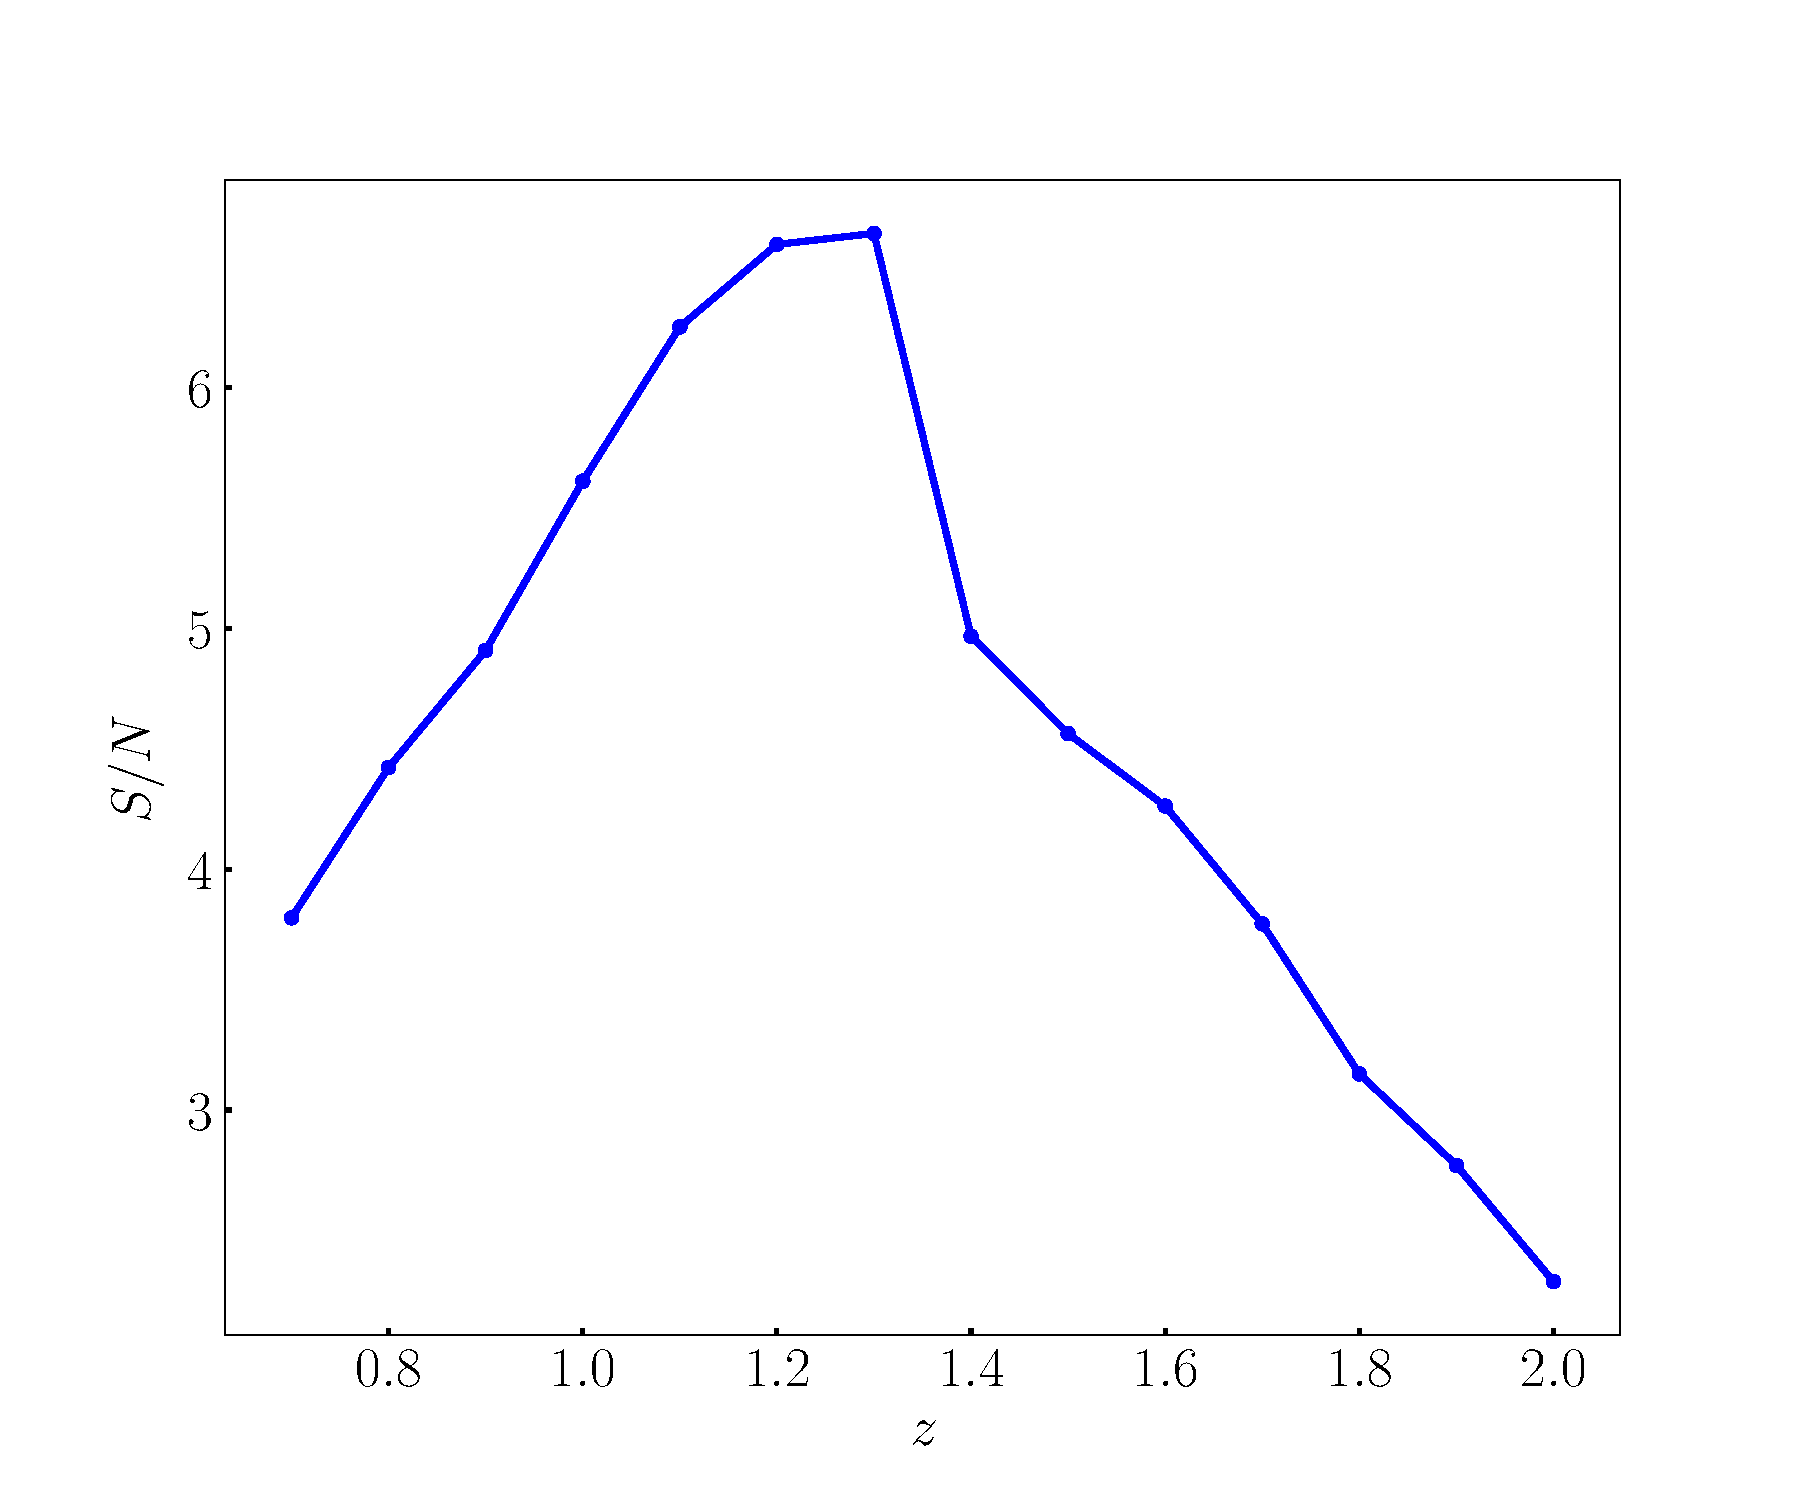
\includegraphics[width=7.5cm]{fig/snrDoppler-eps-converted-to}
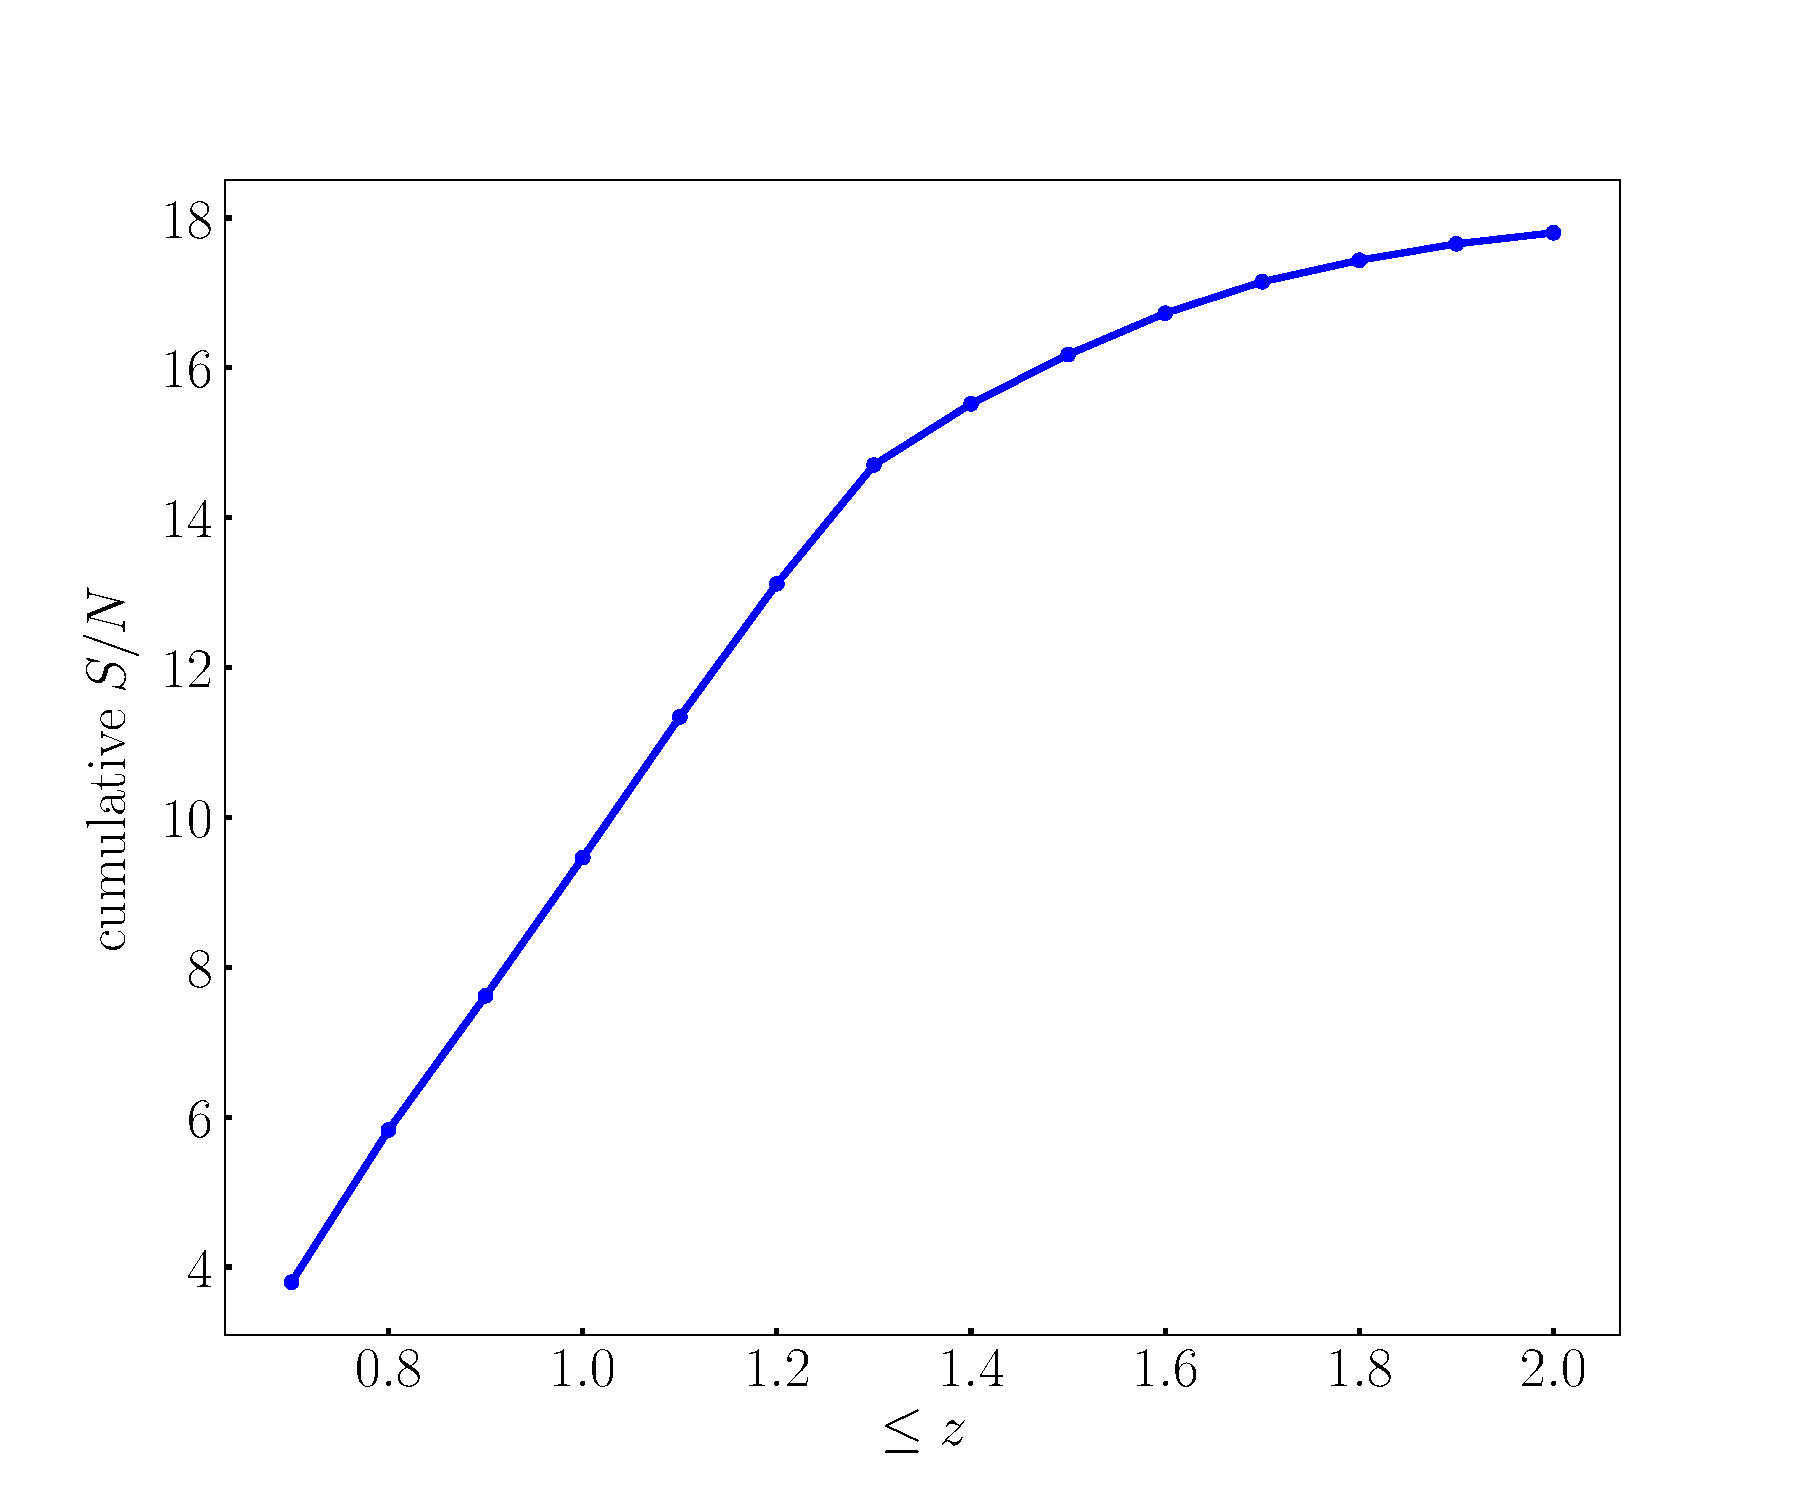
\includegraphics[width=7.5cm]{fig/CumulativesnrDoppler-eps-converted-to}
\caption{Relativistic SNR per $z$-bin  ({\em left}) and cumulative ({\em right}) for a Stage IV $H\alpha$ survey.} \label{fig4}
\end{figure}
\begin{figure}[ht]
\centering
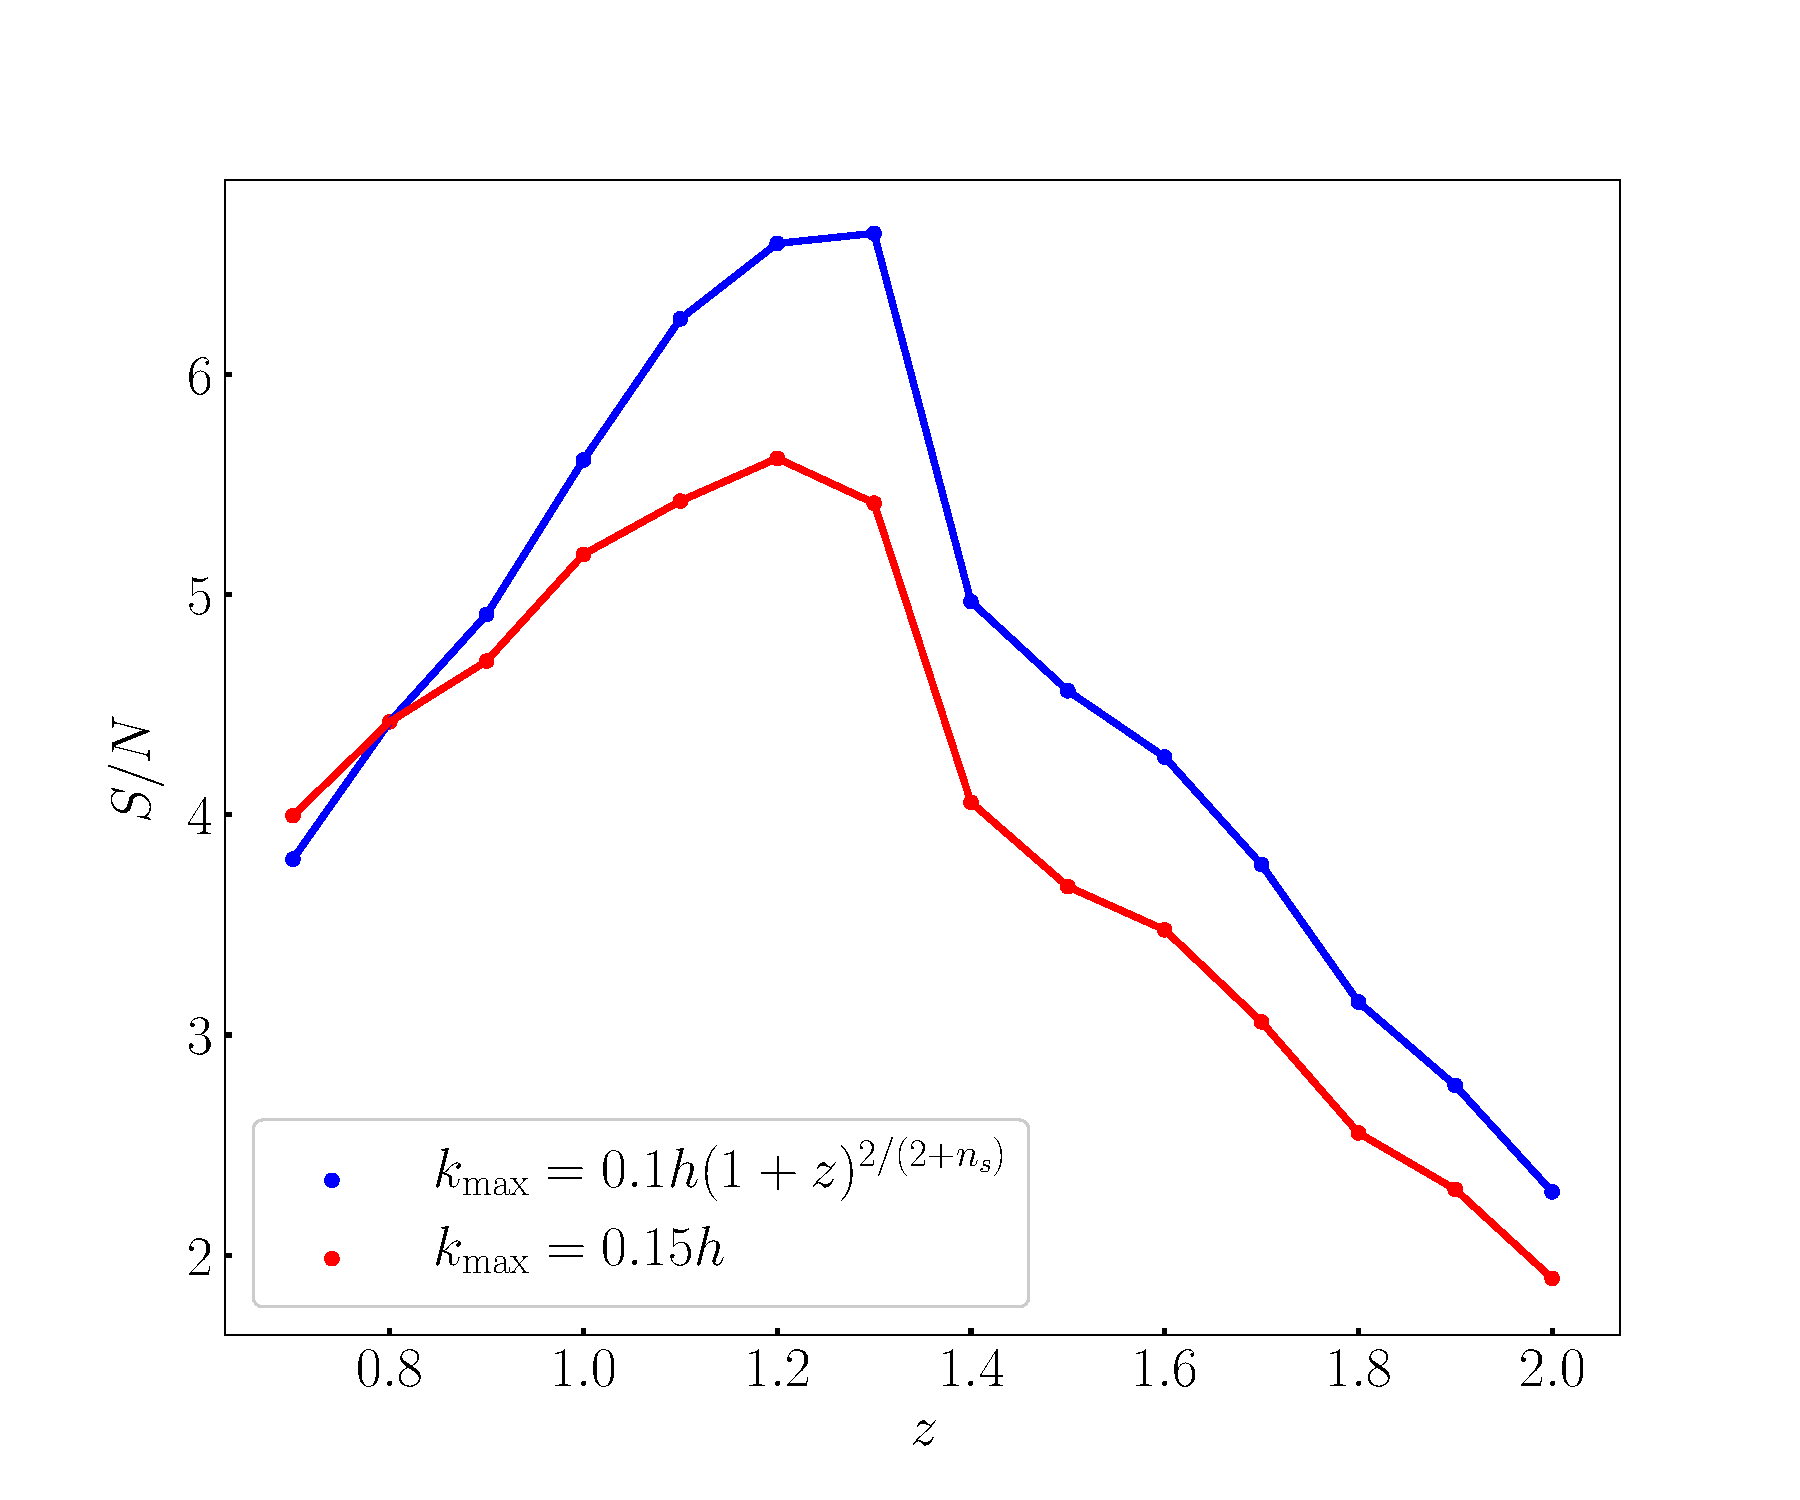
\includegraphics[width=7.5cm]{fig/kmaxsnr-eps-converted-to}
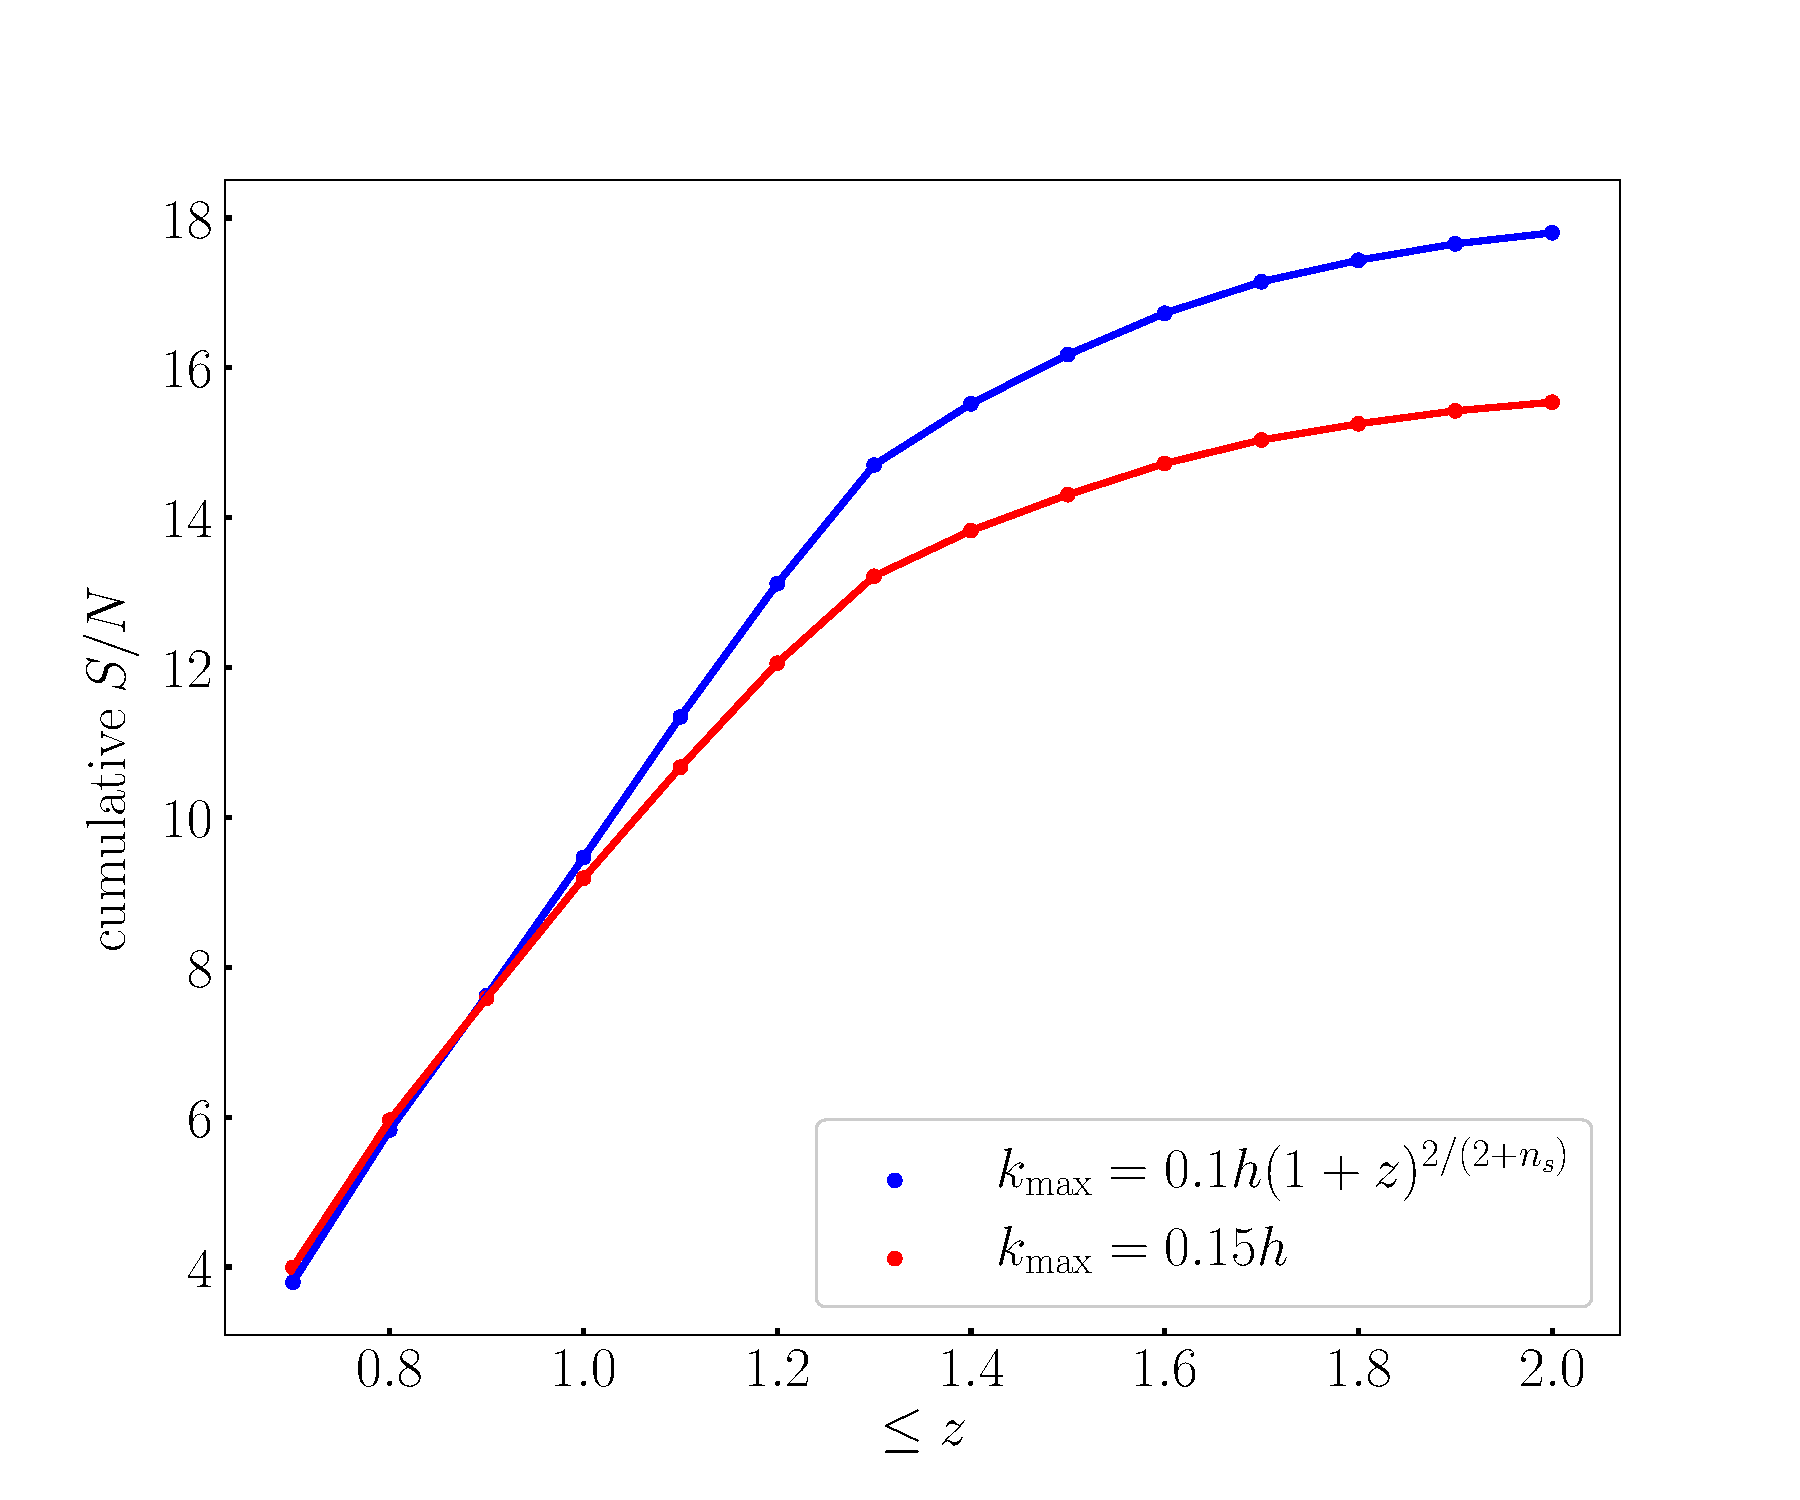
\includegraphics[width=7.5cm]{fig/kmaxcumsnr-eps-converted-to} 
\caption{Effect of changing $k_{\mathrm{max}}$ on SNR per bin ({\em left}) and cumulative SNR ({\em right}).} \label{kmsnr}
\end{figure} 
\item  
Changes in $b_e(z),\Q(z)$: In the Appendix (Fig.~\ref{fig1x}) we  illustrate the significant impact on cumulative SNR of changing $b_e,\Q$. We use a range of constant choices for $b_e,\Q$ -- which are not physically motivated. This shows the importance of modelling $b_e,\Q$ self-consistently from the same  luminosity function that produces the number density, as we have done. 
\end{itemize}

{The sensitivity of the relativistic SNR to  $k_{\mathrm{max}}$ reflects the importance of the coupling of the relativistic signal to Newtonian terms on short scales. How sensitive is the SNR to the signal on the largest scales? We can answer this by increasing $k_{\mathrm{min}}$ from its fiducial value $k_{\mathrm{f}}$, which is the maximal observable scale. The result is that there is only a small reduction when $k_{\mathrm{min}}/k_{\mathrm{f}}$ is increased by a factor up to 5, as shown in Fig.~\ref{kmin}. 
{Even with $k_{\mathrm{min}}=10 k_{\mathrm{f}}$, the total SNR is $\sim 10$.} 
This means that the relativistic SNR does not depend critically on accessing the largest possible scales.}
\begin{figure}[ht]
\centering
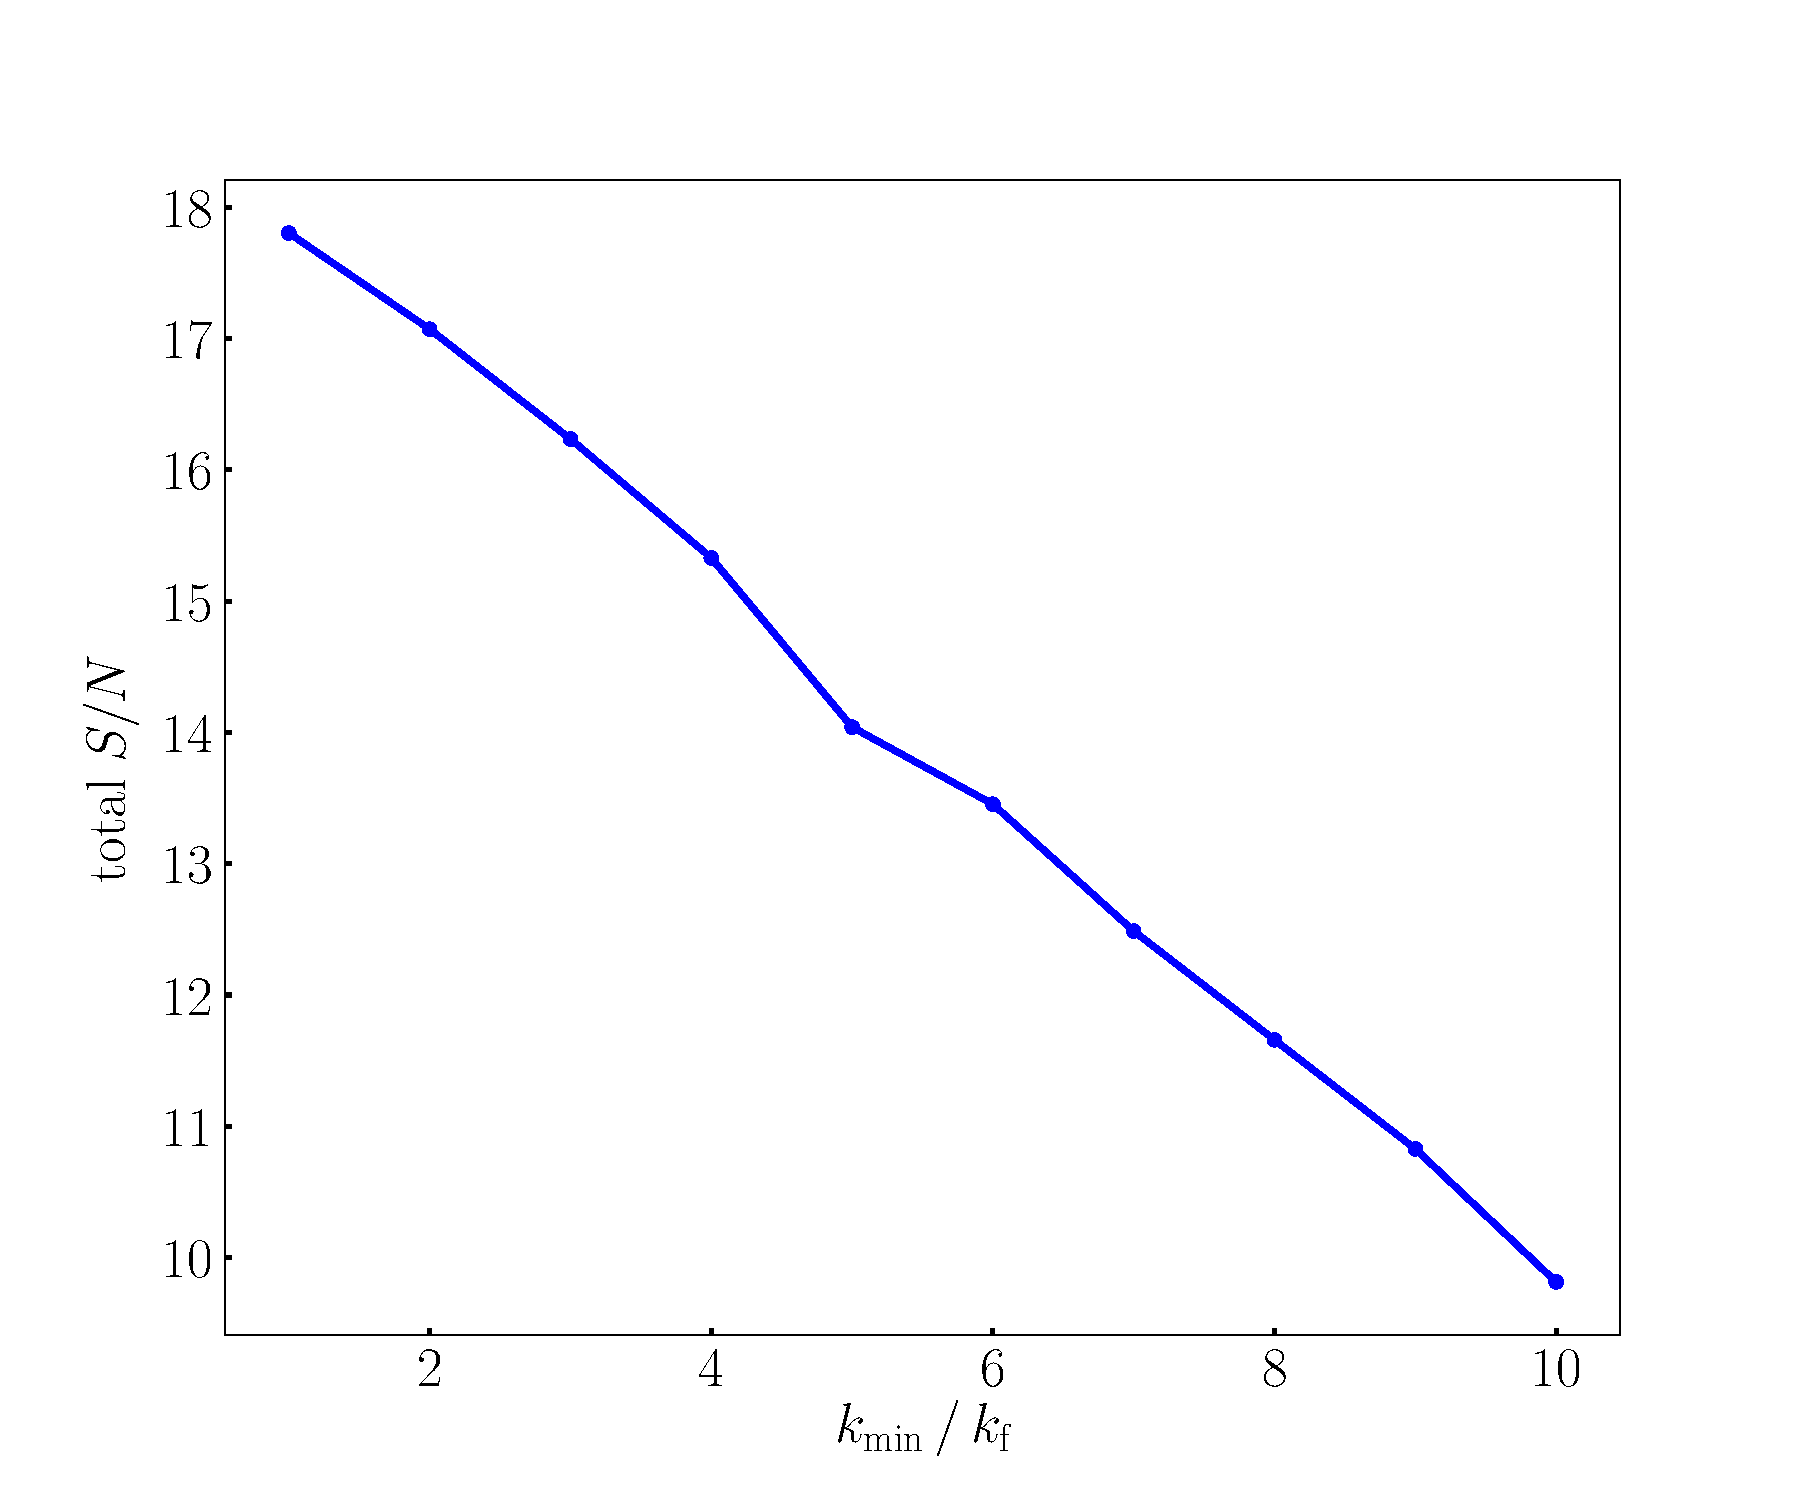
\includegraphics[width=8.0cm]{fig/cumDoppSnr_kmin-eps-converted-to}
\caption{{Effect of changing $k_{\mathrm{min}}$ on  total relativistic SNR.} 
} \label{kmin}
\end{figure} 

It is also interesting to investigate how important for the SNR is the second-order relativistic contribution 
in the bispectrum, i.e. from terms of the form
\begin{equation} \label{2oc}
\mathcal{K}^{(1)}_{\mathrm{N}}(\bm{k}_{1})\mathcal{K}^{(1)}_{\mathrm{N}}(\bm{k}_{2})\mathcal{K}^{(2)}_{\mathrm{D}}(\bm{k}_{1},\bm{k}_{2},\bm{k}_{3})\,,
\end{equation}
 in \eqref{e21},  compared to the first-order contribution, i.e. from terms of the form
 \begin{equation} \label{1oc}
 \Big[\mathcal{K}^{(1)}_{\mathrm{N}}(\bm{k}_{1})\mathcal{K}^{(1)}_{\mathrm{D}}(\bm{k}_{2}) + \mathcal{K}^{(1)}_{\mathrm{D}}(\bm{k}_{1})\mathcal{K}^{(1)}_{\mathrm{N}}(\bm{k}_{2})\Big]\mathcal{K}^{(2)}_{\mathrm{N}}(\bm{k}_{1},\bm{k}_{2},\bm{k}_{3}) \,.
 \end{equation}
 It is conceivable that the first-order Doppler-type contribution in \eqref{1oc} to $B_g$, which couples to first- and second-order Newtonian terms, dominates the SNR. However, we find that the first- and  second-order relativistic parts of the bispectrum make comparable contributions to the SNR -- see Fig.~\ref{fig4z}. We deduce that the second-order relativistic contribution in \eqref{2oc} cannot be neglected. Furthermore, this means that it must be accurately modelled, as we  have done. 
\begin{figure}[ht]
\centering
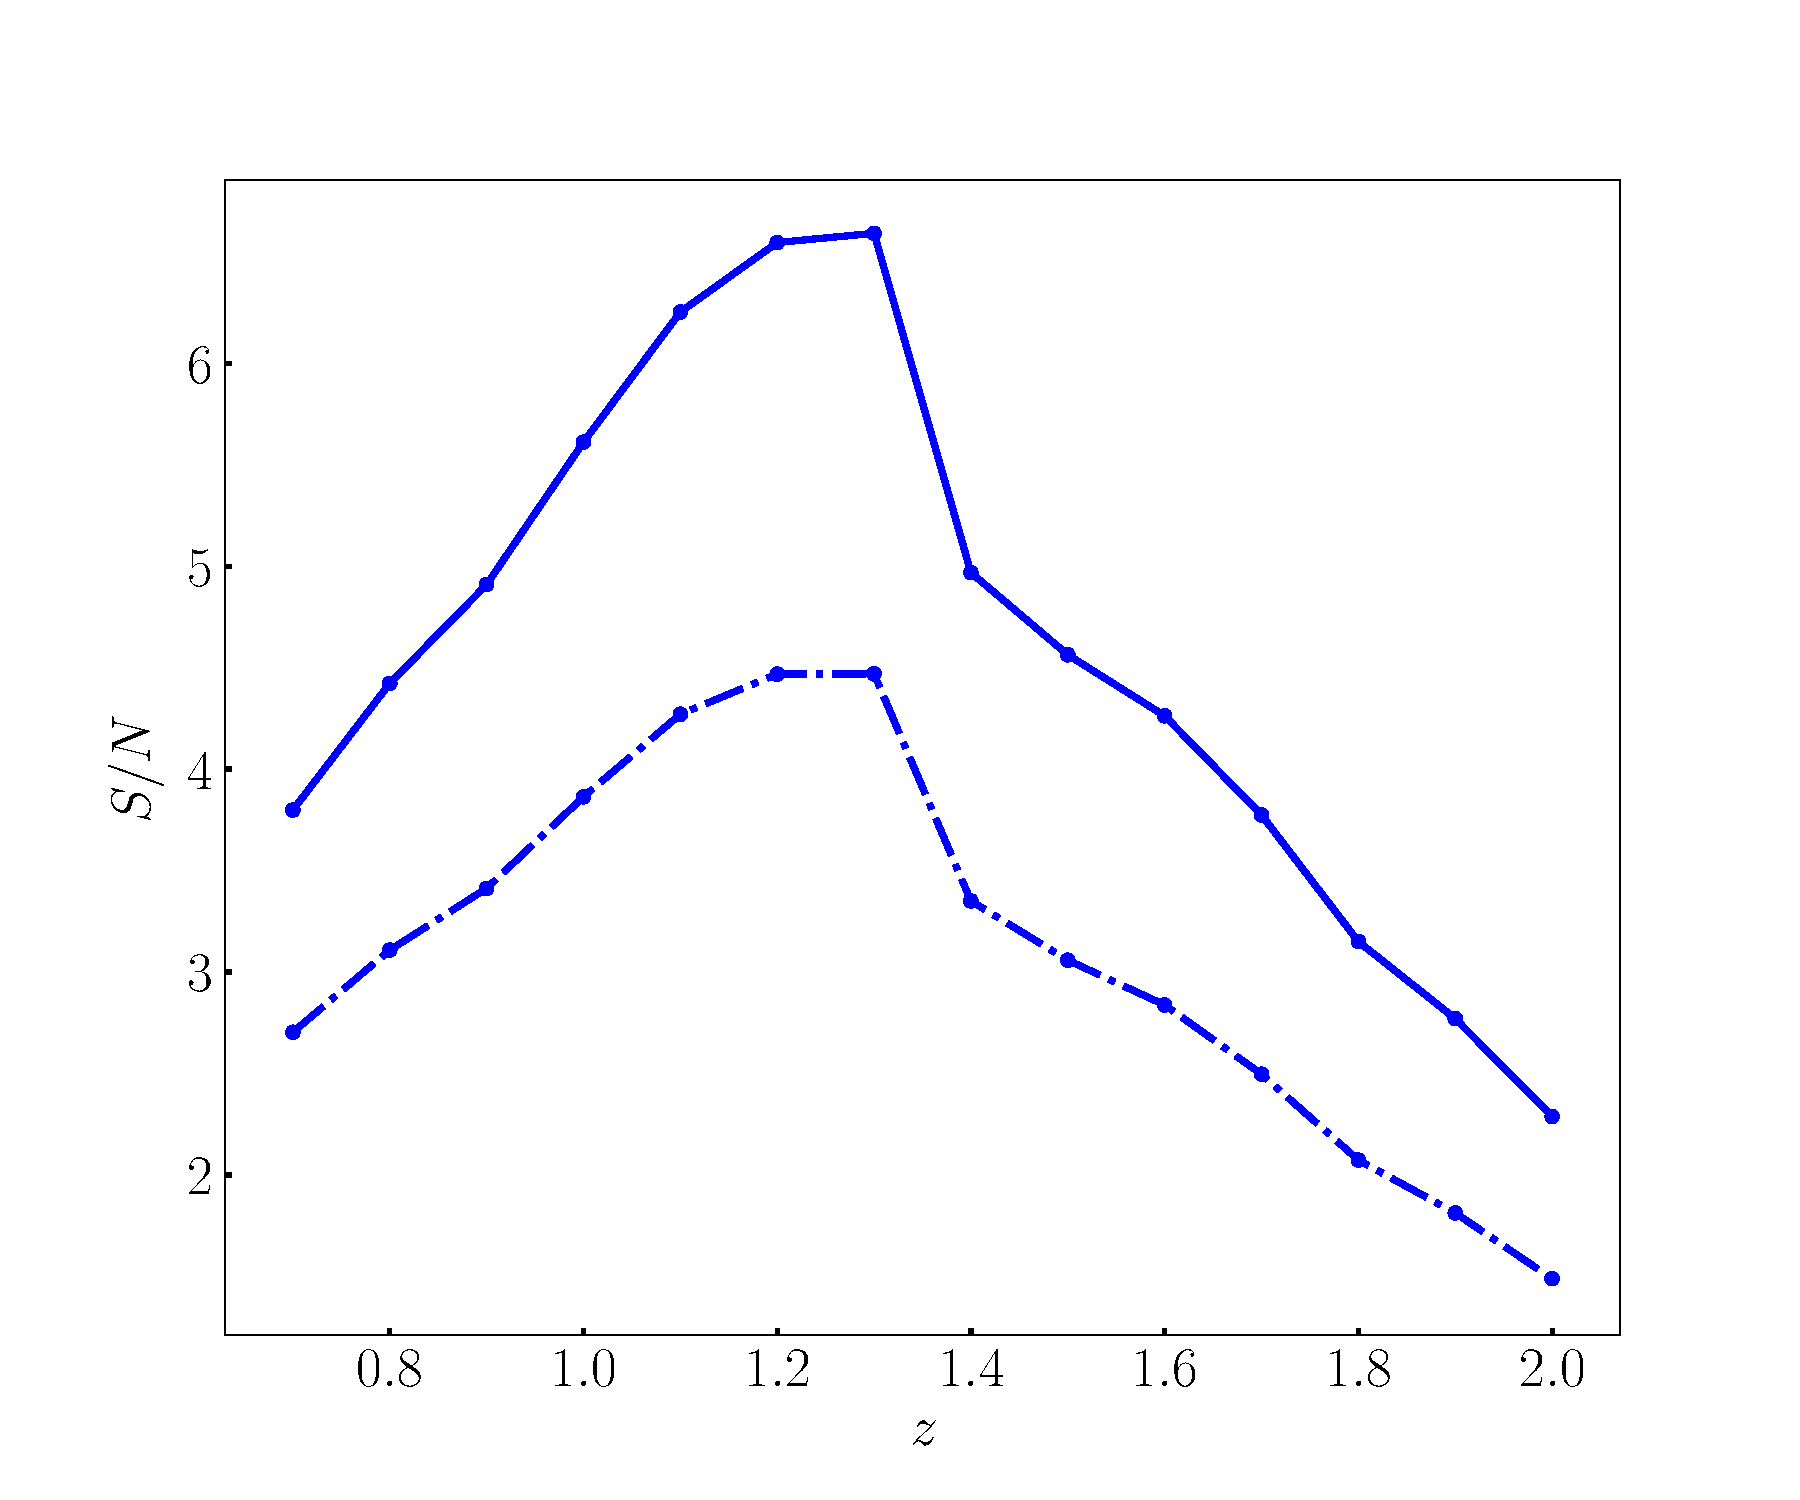
\includegraphics[width=7.5cm]{fig/DoppSnr_K2D-eps-converted-to}
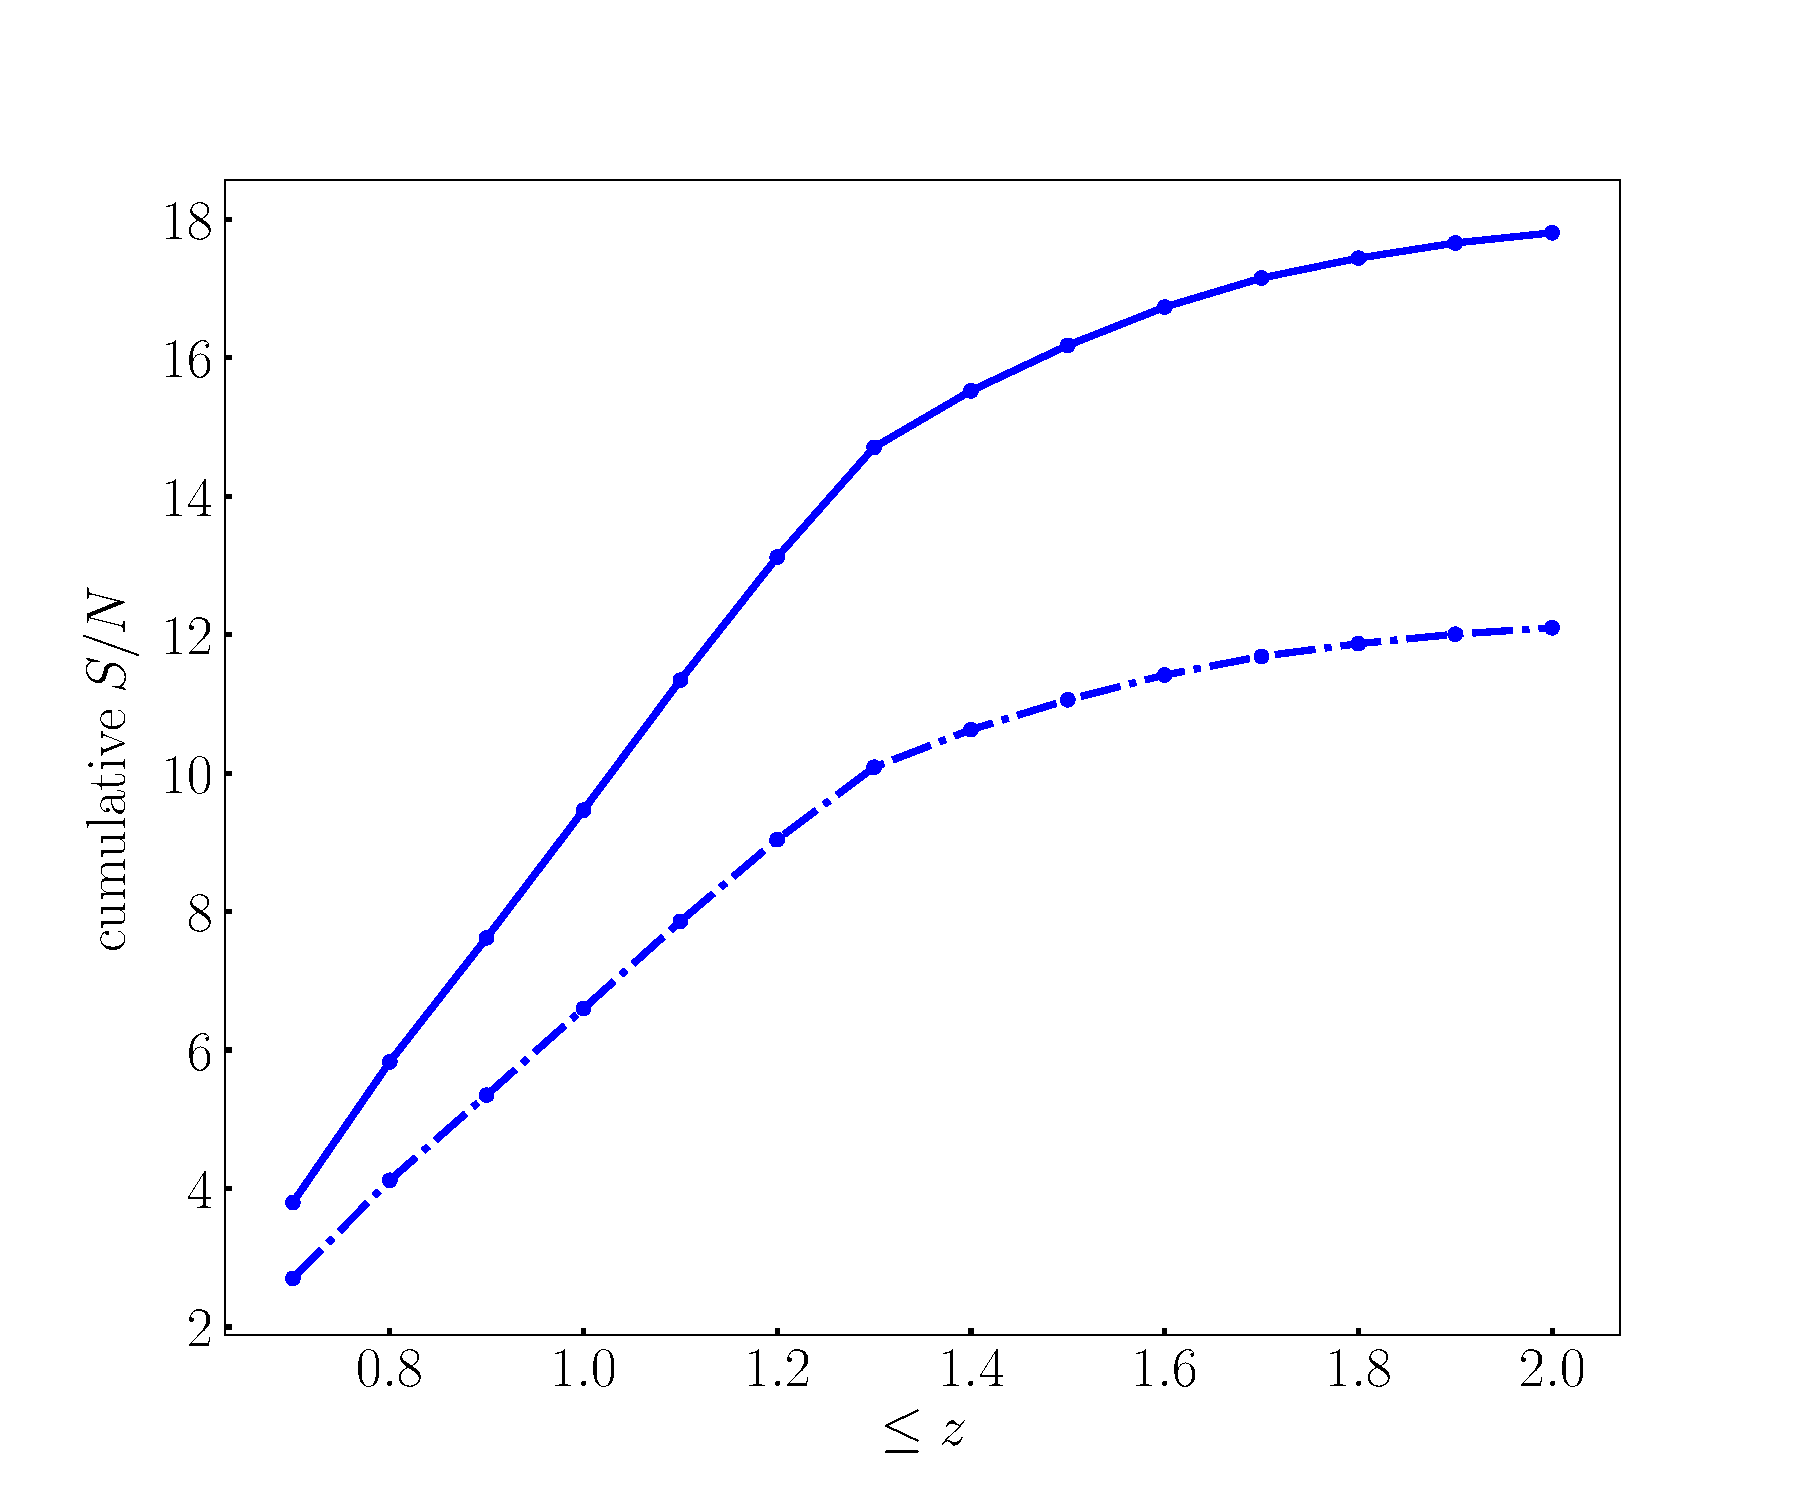
\includegraphics[width=7.5cm]{fig/cumDoppSnr_K2D-eps-converted-to}
\caption{As in Fig.~\ref{fig4}, but showing the effect of omitting the second-order relativistic contribution \eqref{2oc} to the bispectrum (dot-dashed curves).} \label{fig4z}
\end{figure}

Recently \cite{Jeong:2019igb} estimated the  SNR for the leading relativistic part of the bispectrum.  There are significant differences in their analysis compared to ours. In particular, they neglect most of the terms in $\delta_{g \mathrm{D}}^{(2)}$ [see our \eqref{dg2}] which defines ${\cal K}^{(2)}_{\mathrm{D}}$ (see the Appendix for further details). {In addition they do not use self-consistent models for $b_{e}$ and $\mathcal{Q}$. These two differences could account for their conclusion that the relativistic signal is not detectable, in contrast to our result.} 

An interesting feature of the relativistic signal is that there is a significant contribution to the SNR from  flattened triangle shapes. This is consistent with the results of  \cite{Clarkson:2018dwn} for the dipole that is generated by the imaginary part of the bispectrum.
%
%
\subsection{Including cosmological parameters}
~\\
%
%----------------------------------------------
%
%
\section{{Conclusions}}
